\chapter{Dasar Teori}
\label{chap:dasar_teori}

\section{MySQL Spatial Extensions}
\label{sec:mysql_spatial_ex}
	Suatu \textit{geographic feature}\cite{mysqlspatial} adalah sesuatu yang ada di bumi yang memiliki lokasi sebagai penunjuk letak keberadaannya. Geometri adalah cabang ilmu matematika yang digunakan untuk memodelkan suatu \textit{geographic feature}. Dengan geometri, suatu \textit{geographic feature} dapat dinyatakan sebagai sebuah titik, garis, ruang, ataupun bentuk lainnya. Suatu ``\textit{feature}'' yang dimaksud dalam istilah \textit{geographic feature} dapat berupa:
	\begin{enumerate}
		\item \textbf{\textit{An entity}}, contohnya adalah gunung, kolam, kota, dll.
		\item \textbf{\textit{A space}}, contohnya adalah daerah, cuaca, dll.
		\item \textbf{\textit{A definable location}}, contohnya adalah persimpangan jalan, yaitu suatu tempat khusus dimana terdapat 2 buah jalan yang saling berpotongan.
	\end{enumerate}
	
	MySQL adalah salah satu perangkat lunak yang digunakan untuk mengatur data-data (\textit{database}) suatu situs web. Bentuk MySQL adalah sekumpulan tabel yang umumnya memiliki hubungan antar satu dengan yang lainnya. Setiap tabel pada MySQL memiliki kolom dan baris. Kolom pada MySQL menyatakan daftar jenis baris yang ingin dibuat dan baris menyatakan banyaknya data yang ada dalam tabel.
	
	Penamaan suatu kolom dalam MySQL membutuhkan penentuan tipe data yang akan digunakan dalam kolom tersebut. Dalam MySQL terdapat tipe-tipe data yang umum digunakan seperti \textit{Varchar} untuk menyimpan karakter atau kata, \textit{Int} untuk menyimpan angka, \textit{Boolean} untuk menyimpan nilai ``\texttt{true}'' atau ``\texttt{false}'', dan tipe data lainnya. MySQL Spatial Extensions adalah perluasan dari tipe-tipe data yang disediakan MySQL untuk menyatakan nilai geometri dari suatu \textit{geographic feature}.
	
	Berdasarkan kemampuan penyimpanan nilai geometri, tipe data \textit{spatial} dapat dikelompokan ke dalam 2 jenis:
\begin{enumerate}
	\item Tipe data yang hanya dapat menyimpan sebuah nilai geometri saja, yaitu:
	\begin{itemize}
		\item \textbf{\textit{Geometry}}
		\item \textbf{\textit{Point}}
		\item \textbf{\textit{LineString}}
		\item \textbf{\textit{Polygon}}
	\end{itemize}
	\item Tipe data yang dapat menyimpan sekumpulan nilai geometri, yaitu:
	\begin{itemize}
		\item \textbf{\textit{MultiPoint}}
		\item \textbf{\textit{MultiLineString}}
		\item \textbf{\textit{MultiPolygon}}
		\item \textbf{\textit{GeometryCollection}}
	\end{itemize}
\end{enumerate}

\subsection{\textit{Point}}
\label{sec:point}
\textit{Point} adalah nilai geometri yang merepresentasikan sebuah lokasi ke dalam suatu koordinat\cite{mysqlspatial}. Koordinat pada \textit{Point} terdiri dari nilai X dan Y dimana X merepresentasikan letak lokasi terhadap garis bujur dan Y merepresentasikan letak lokasi terhadap garis lintang. \textit{Point} tidak memiliki dimensi maupun nilai batasan. Contoh representasi \textit{Point} adalah Universitas Katolik Parahyangan direpresentasikan dalam koordinat X=107.6049079 dan Y=-6.874735 (gambar \ref{fig:2_UNPAR}).

\begin{figure}[htbp]
	\centering
		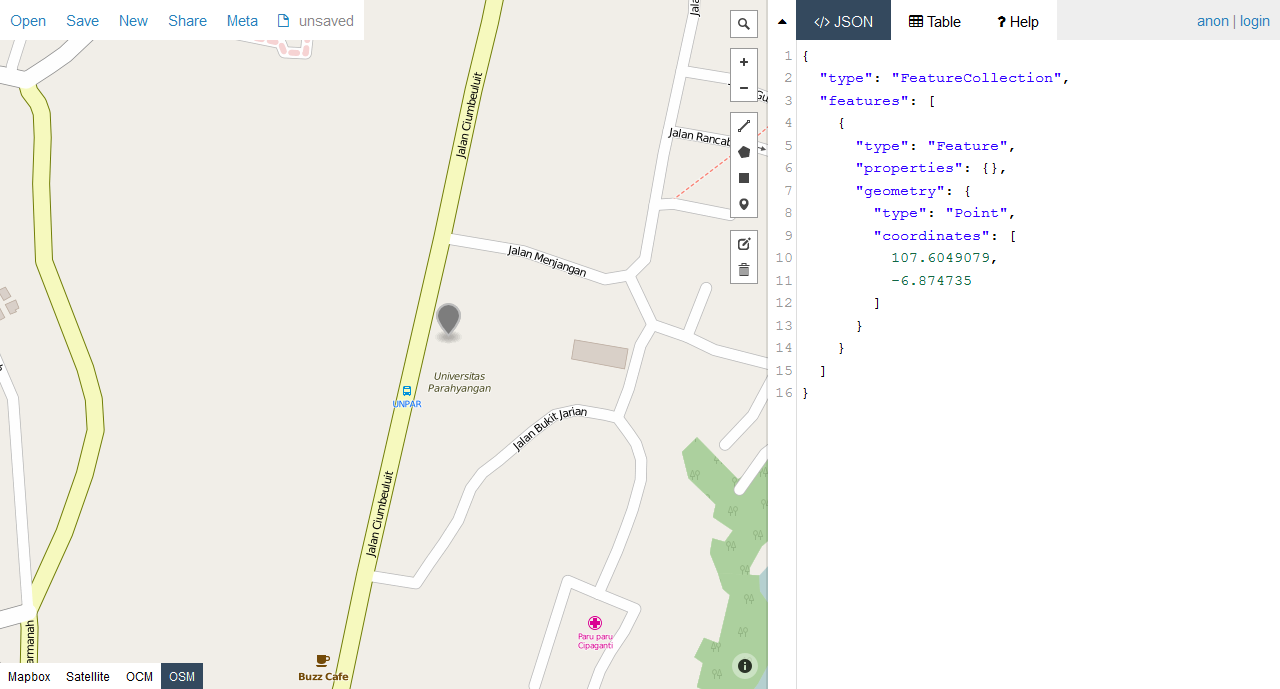
\includegraphics[scale=0.35]{Gambar/2_point.png}
	\caption{Universitas Katolik Parahyangan dinyatakan dalam \textit{Point}\cite{geojson}}
	\label{fig:2_UNPAR}
\end{figure}

\subsection{\textit{LineString}}
\label{sec:linestring}
\textit{LineString} adalah garis yang terbentuk dari sekumpulan \textit{Point}\cite{mysqlspatial}. Dalam peta dunia, \textit{LineString} dapat merepresentasikan sebuah sungai dan dalam peta perkotaan, \textit{LineString} dapat merepresentasikan sebuah jalan (contoh: gambar \ref{fig:2_linestring}). Karena \textit{LineString} merupakan sekumpulan \textit{Point}, maka \textit{LineString} menyimpan sekumpulan koordinat dimana setiap koordinat ($X_{1}$\ldots$X_{n}$ dan $Y_{1}$\ldots$Y_{n}$, dimana n menyatakan banyaknya \textit{Point} dalam \textit{LineString}) terhubung oleh garis dengan koordinat selanjutnya. Contohnya: misal terdapat sebuah \textit{LineString} yang mengandung 3 buah \textit{Point}, maka terdapat garis yang menghubungkan \textit{Point} pertama dengan \textit{Point} kedua dan \textit{Point} kedua dengan \textit{Point} ketiga.

\begin{figure}[htbp]
	\centering
		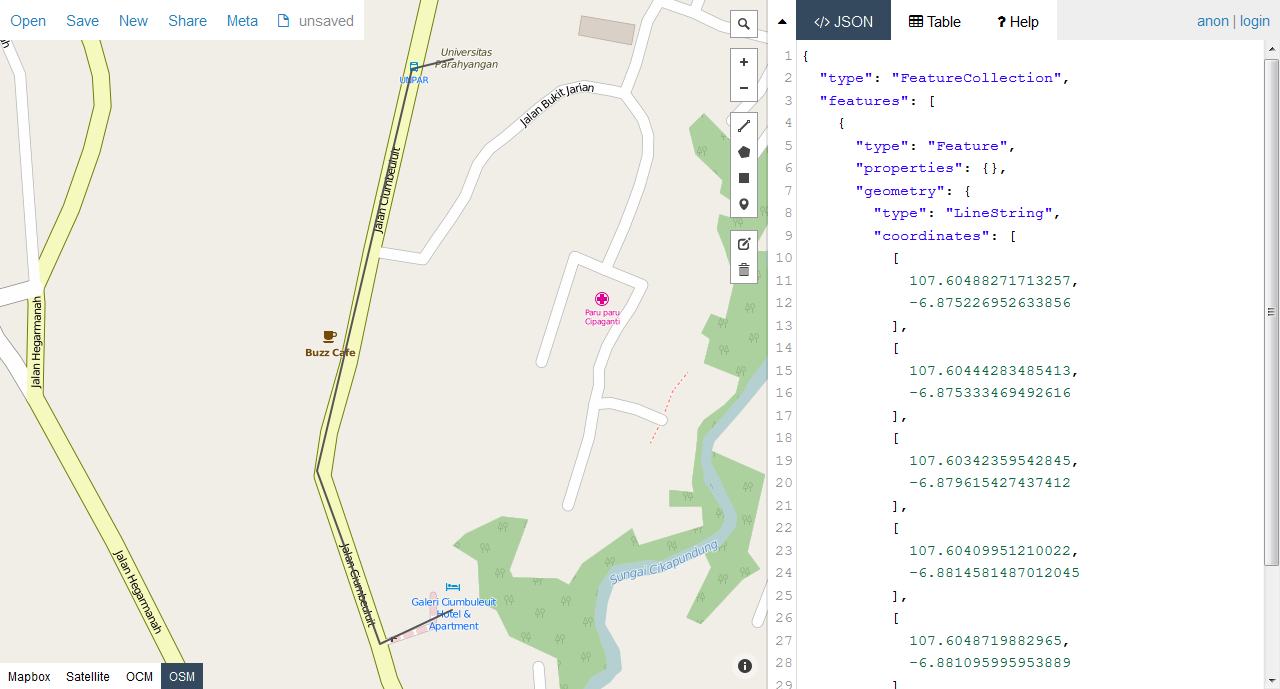
\includegraphics[scale=0.35]{Gambar/2_linestring.png}
	\caption{Rute jalan dari Universitas Katolik Parahyangan menuju Galeri Ciumbuleuit dinyatakan dalam \textit{LineString}\cite{geojson}}
	\label{fig:2_linestring}
\end{figure}

\subsection{Format Well-Known Text (WKT)}
\label{sec:wktformat}
Format Well-Known Text (WKT) adalah salah satu aturan penulisan tipe data \textit{spatial} untuk merepresentasikan suatu \textit{geographic feature}\cite{mysqlspatial}. WKT merepresentasikan nilai geometri yang dimodelkan untuk pertukaran data geometri dalam ASCII \textit{form}. Berikut adalah contoh format WKT:

\begin{lstlisting}
	POINT(107.6049079 -6.874735)
	
	LINESTRING(107.60502219200134 -6.875194997571583, 
						 107.60445356369019 -6.875386727913034,
						 107.60347723960876 -6.879647382202341,
						 107.6040780544281 -6.881479451795388,
						 107.60461449623108 -6.8812344661545986,
						 107.60483980178833 -6.880861661676069)
\end{lstlisting}

Contoh di atas menunjukkan format WKT dari \textit{Point} (baris 1) dan format WKT dari \textit{LineString} (baris 3-8).

Berikut adalah contoh penggunaan format WKT dalam MySQL:

\begin{lstlisting}
	CREATE TABLE geom (g LINESTRING);

	INSERT INTO geom VALUES (ST_GeomFromText('LINESTRING(107.60502219200134 -6.875194997571583, 
						 107.60445356369019 -6.875386727913034,
						 107.60347723960876 -6.879647382202341,
						 107.6040780544281 -6.881479451795388,
						 107.60461449623108 -6.8812344661545986,
						 107.60483980178833 -6.880861661676069)'));
	
	SELECT ST_AsText(g) FROM geom;
\end{lstlisting}

Contoh di atas menunjukkan pembuatan tabel ``\texttt{geom}'' dengan sebuah kolom ``\texttt{g}'' dan tipe data ``\texttt{LINESTRING}'' (baris 1), menambahkan 1 baris data berupa \textit{LineString} ke dalam tabel ``\texttt{geom}'' (baris 3-8), dan melihat data dari tabel ``\texttt{geom}'' (baris 10), dimana nilai kembalian ``\texttt{ST\_AsText(g)}'' berupa data \textit{LineString} dalam format WKT .



\section{JDBC}
\label{sec:jdbc}
JDBC API adalah bagian dari Java API yang dapat digunakan untuk mengakses semua jenis data yang terstruktur, terutama data yang tersimpan dalam suatu \textit{Relational Database}\cite{javadocumentation}. JDBC dapat membantu 3 jenis aktivitas \textit{programming} dalam menggunakan bahasa Java, yaitu:
\begin{enumerate}
	\item Menghubungkan aplikasi Java ke suatu sumber data seperti \textit{database},
	\item Mengirimkan \textit{queries} dan pembaharuan \textit{statement} ke \textit{database},
	\item Menerima dan melakukan proses terhadap hasil yang didapatkan dari pengiriman \textit{queries} tersebut.
\end{enumerate}
Berikut adalah contoh struktur kode yang mewakili 3 jenis aktivitas yang dapat dilakukan JDBC API:

\begin{lstlisting}
public void connectToAndQueryDatabase(String username, String password) {

    Connection con = DriverManager.getConnection(
                         "jdbc:myDriver:myDatabase",
                         username,
                         password);

    Statement stmt = con.createStatement();
    ResultSet rs = stmt.executeQuery("SELECT a, b, c FROM Table1");

    while (rs.next()) {
        int x = rs.getInt("a");
        String s = rs.getString("b");
        float f = rs.getFloat("c");
    }
}
\end{lstlisting}

Contoh di atas menunjukkan bagaimana JDBC API membantu aplikasi Java membuat koneksi terhadap suatu \textit{database} (baris 3-6), membuat dan mengirimkan suatu \textit{query} ke \textit{database} (baris 8 dan 9), dan menerima dan melakukan proses terhadap hasil yang didapatkan dari pengiriman \textit{query} tersebut (baris 9-15).

\subsection{\textit{Interface} Connection}
\label{sec:intercon}
\textit{Interface} Connection adalah sebuah koneksi (\textit{session}) dengan \textit{database} spesifik\cite{javadocumentation}. Eksekusi SQL \textit{statements} (subbab \ref{sec:statement}) dan penerimaan hasil kembalian (subbab \ref{sec:resultset}) dari eksekusi tersebut dapat terjadi karena adanya koneksi dengan \textit{database} yang dibentuk oleh \textit{interface} Connection. Berikut adalah sebagian \textit{method} yang ada pada \textit{interface} Connection:
\begin{itemize}
	\item \texttt{void close()}
	
	\textit{Method} ini digunakan untuk memutuskan koneksi dengan \textit{database} yang sedang terhubung.
	
	\item \texttt{Statement createStatement()}
	
	\textit{Method} ini digunakan untuk membangun objek \texttt{Statement} yang dapat digunakan untuk mengirimkan SQL \textit{statements} ke \textit{database} yang sedang terhubung.
\end{itemize}

\subsection{Kelas DriverManager}
\label{sec:drivermanager}
Kelas DriverManager adalah cara paling dasar untuk mengatur JDBC \textit{drivers}\cite{javadocumentation}. Berikut adalah salah satu \textit{method} yang ada di kelas DriverManager untuk mengatur JDBC \textit{drivers}:
\begin{itemize}
	\item \texttt{public static Connection getConnection(String url, String user, String password)}
	
	\textit{Method} ini digunakan untuk membangun sebuah koneksi dengan \textit{database}. Umumnya method ini digunakan untuk membangun \textit{interface} Connection (subbab \ref{sec:intercon}).
	
	Parameter:
	\begin{enumerate}
		\item \texttt{url}, alamat dari \textit{database}, formatnya adalah ``\textit{jdbc:\textit{subprotocol}:\textit{subname}}'',
		\item \texttt{user}, \textit{username} untuk mengakses \textit{database},
		\item \texttt{password}, \textit{password} dari \textit{username}.
	\end{enumerate}
	
	Nilai kembalian: sebuah koneksi terhadap \textit{database} yang sesuai dengan alamat \texttt{url}.
\end{itemize}

\subsection{\textit{Interface} Statement}
\label{sec:statement}
\textit{Interface} Statement adalah objek yang digunakan untuk melakukan eksekusi terhadap suatu \textit{query} dan mengembalikan nilai kembalian dari eksekusi tersebut\cite{javadocumentation}. Berikut adalah salah satu \textit{method} yang ada di \textit{interface} Statement:
\begin{itemize}
	\item \texttt{ResultSet executeQuery(String sql)}
	
	Parameter: \texttt{sql}, sebuah SQL \textit{statement} yang akan dikirimkan ke \textit{database}.
	
	Nilai kembalian: objek \texttt{ResultSet} yang berupa data yang dihasilkan dari eksekusi \textit{query} \texttt{sql}.
\end{itemize}

\subsection{\textit{Interface} ResultSet}
\label{sec:resultset}
\textit{Interface} ResultSet adalah sebuah tabel data yang merepresentasikan hasil dari sebuah eksekusi \textit{query} pada suatu \textit{database}\cite{javadocumentation} (subbab \ref{sec:statement}). Cara kerja \textit{interface} ResultSet adalah dengan sistem indeks. Pada awalnya indeks ResultSet menunjuk pada data ``bayangan'' sebelum data pertama. Setiap pemanggilan \textit{method} ``\texttt{next()}'' pada objek ResultSet akan menyebabkan nilai indeks semakin meningkat (bertambah 1). Berikut adalah contoh \textit{method} \textit{interface} ResultSet:
\begin{itemize}
	\item \texttt{boolean next()}
	
	Nilai kembalian: \texttt{true} jika terdapat data pada indeks selanjutnya, \texttt{false} bila tidak ditemukan data pada indeks selanjutnya.

	\item \texttt{Object getObject(String columnLabel)}
	
	Parameter: \texttt{columnLabel}, merupakan nama kolom yang ingin diambil nilainya.
	
	Nilai kembalian: data berupa \texttt{Object} pada indeks baris dan kolom yang ditunjuk.
	
	\item \texttt{String getString(String columnLabel)}
	
	Parameter: \texttt{columnLabel}, merupakan nama kolom yang ingin diambil nilainya.
	
	Nilai kembalian: data berupa \texttt{String} pada indeks baris dan kolom yang ditunjuk.
	
	\item \texttt{int getInt(String columnLabel)}
	
	Parameter: \texttt{columnLabel}, merupakan nama kolom yang ingin diambil nilainya.
	
	Nilai kembalian: data berupa \texttt{int} pada indeks baris dan kolom yang ditunjuk.
	
	\item \texttt{boolean getBoolean(String columnLabel)}
	
	Parameter: \texttt{columnLabel}, merupakan nama kolom yang ingin diambil nilainya.
	
	Nilai kembalian: data berupa \texttt{boolean} pada indeks baris dan kolom yang ditunjuk.
\end{itemize}



\section{Play Framework}
\label{sec:play_framework}
Play Framework adalah sekumpulan kerangka kode yang dapat digunakan untuk membangun suatu situs web\cite{playforjava}. Play Framework tidak hanya menggunakan bahasa Java dalam pembuatannya. Bahasa Scala juga digunakan Play Framework dalam beberapa bagian seperti bagian \textit{view} dan \textit{route}. Play Framework menggunakan konsep MVC (\textit{Model} \textit{View} \textit{Controller}) sebagai pola arsitekturnya. Konsep MVC pada suatu kode membuat kode mudah dikembangkan baik secara tampilan maupun pengembangan fitur-fiturnya. Ketika \textit{server} Play Framework dijalankan, secara \textit{default} dapat diakses melalui ``localhost:9000''.

\subsection{Struktur Aplikasi}
\label{sec:struktur_aplikasi}
Ketika Play Framework pertama kali ter-\textit{install} pada komputer, Play Framework menyediakan \textit{default} direktori dengan struktur minimal (gambar \ref{fig:2_strukturplay}). Berikut adalah penjelasan struktur minimal Play Framework:
\begin{enumerate}
	\item \textit{Folder} ``app'' merupakan \textit{folder} yang berisi mengenai pola arsitektur yang dimiliki Play Framework, yaitu ``models'' (tidak dibuat secara \textit{default}), ``views'', dan ``controllers'' yang akan dijelaskan lebih lanjut pada subbab selanjutnya (subbab \textit{Models}: \ref{sec:models}, subbab \textit{Views}: \ref{sec:views}, dan subbab \textit{Controllers}: \ref{sec:controllers}).
	\item \textit{Folder} ``conf'' berisi mengenai \textit{file} ``application.conf'' yang menyimpan pengaturan-pengaturan seperti kumpulan \textit{log}, koneksi ke \textit{database}, jenis \textit{port} tempat \textit{server} bekerja, dll. \textit{Folder} ``conf'' juga berisi \textit{file} ``routes'' yang mengatur bagaimana HTTP \textit{requests} nantinya akan diproses lebih lanjut yang akan dijelaskan pada subbab selanjutnya (subbab \ref{sec:routes}).
	\item \textit{Folder} ``project'' terdapat \textit{file} ``build.properties'' dan ``plugins.sbt'', \textit{file} tersebut mendeskripsikan versi Play dan SBT yang digunakan pada aplikasi.
	\item \textit{Folder} ``public'' merupakan \textit{folder} yang menyimpan data-data seperti gambar (\textit{folder} ``images''), kumpulan Javascript yang digunakan (\textit{folder} ``javascripts'', secara \textit{default} berisikan \textit{file} ``jquery-1.9.0.min.js'') dan data-data CSS (folder ``stylesheets'').
	\item \textit{File} ``build.sbt'' mengatur \textit{dependencies} yang dibutuhkan dalam pembuatan aplikasi.
	\item Terakhir adalah \textit{folder} ``test'' yang merupakan salah satu kelebihan dari Play Framework, bagian ini berisikan \textit{file} ``Application.test'' dan ``Integration.test'' yang dapat digunakan untuk melakukan serangkaian \textit{testing} yang diinginkan terhadap aplikasi.
\end{enumerate}
     

\begin{figure}[htbp]
	\centering
		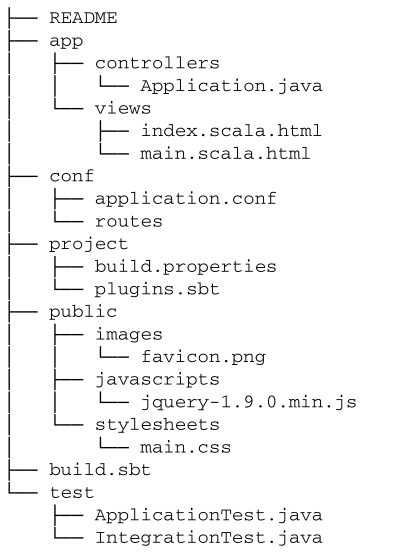
\includegraphics[scale=0.7]{Gambar/2_strukturplay.PNG}
	\caption{Struktur minimal Play Framework}
	\label{fig:2_strukturplay}
\end{figure}

\subsection{\textit{Routes}}
\label{sec:routes}
\textit{Routes} adalah \textit{file} yang mengatur pemetaan dari HTTP URLs menuju kode aplikasi (dalam hal ini menuju ke \textit{controllers}). Secara \textit{default}, \textit{routes} berisikan kode yang dapat memetakan permintaan URL \textit{index} standar seperti ``localhost:9000'' ketika \textit{server} Play Framework sudah dijalankan.

Berikut adalah isi kode \textit{default} \textit{routes}:

\begin{lstlisting}
	# Home page
	GET     /                           controllers.Application.index()

	# Map static resources from the /public folder to the /assets URL path
	GET     /assets/*file               controllers.Assets.at(path="/public", file)
\end{lstlisting}

Contoh di atas menunjukkan bagaimana \textit{routes} memetakan permintaan URL \textit{index} atau ``/'' (baris ke 2) dan permintaan URL ``/assets/*file'' (baris ke 5).

Struktur \textit{routes} terdiri dari 3 bagian (gambar \ref{fig:2_routes}), yaitu HTTP \textit{method}, URL \textit{path}, dan \textit{action method}. Struktur \textit{routes} seperti yang dijelaskan pada gambar \ref{fig:2_routes} juga sekaligus menjadi struktur minimal yang harus ada agar \textit{routes} dapat memetakan suatu HTTP URLs. HTTP \textit{method} berisikan protokol yang ingin dilakukan terhadap suatu HTTP \textit{request}. HTTP \textit{method} dapat berupa ``\texttt{GET}'', ``\texttt{POST}'', ``\texttt{DELETE}'', ``\texttt{PATCH}'', ``\texttt{HEAD}'' atau ``\texttt{PUT}''\cite{playframeworkweb}. URL \textit{path} merupakan direktori yang ingin dituju dalam \textit{server} aplikasi. URL \textit{path} dimulai dengan tanda ``/'' dan diikuti dengan nama direktori yang ingin dituju. Terakhir, \textit{action method} merupakan pemilihan kelas \textit{controller} yang ingin dituju. Struktur \textit{action method} terdiri dari 3 bagian (dipisahkan dengan karakter ``.''), yaitu pemilihan \textit{package} ``controllers'' yang ingin dituju, bagian kedua adalah pemilihan kelas ``controllers'' yang dipilih (contohnya: ``Products'' pada gambar \ref{fig:2_routes}), dan terakhir adalah pemilihan \textit{method} yang ada pada kelas ``controllers'' yang dipilih (contohnya: ``list()'').

\begin{figure}[htbp]
	\centering
		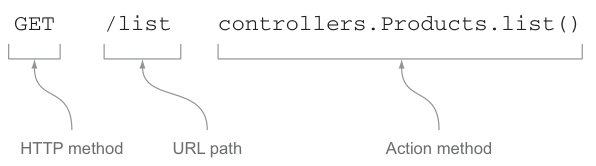
\includegraphics[scale=0.8]{Gambar/2_routes.PNG}
	\caption{Struktur kode \textit{file} ``routes''\cite{playforjava}}
	\label{fig:2_routes}
\end{figure}

URL \textit{path} dan \textit{action method} pada \textit{routes} juga dapat berisi sebuah nilai variabel. Berikut adalah contoh penulisan program URL \textit{path} dan \textit{action method} pada \textit{routes} yang berisi sebuah nilai variabel:

\begin{lstlisting}
	GET   /clients/:id          controllers.Clients.show(id: Long)
\end{lstlisting}

Penulisan sebuah variabel pada URL \textit{path} dimulai dengan tanda ``:'' lalu diikuti dengan nama variabel yang diinginkan, contohnya: ``\texttt{:id}''. Ketika menggunakan variabel pada URL \textit{path}, pada \textit{action method} perlu ditambahkan deklarasi variabel yang diletakan di dalam bagian \textit{method} yang dipilih. Cara penulisan deklarasi variabel pada \textit{action method} adalah dimulai dengan nama variabel, lalu diikuti karakter ``:'', dan diakhiri dengan tipe variabel yang diinginkan. Contoh penulisan deklarasi variabel di dalam \textit{method} suatu kelas pada bagian \textit{action method} adalah ``\texttt{id: Long}''. 

\subsection{\textit{Models}}
\label{sec:models}
Fungsi \textit{models} pada Play Framework sama seperti fungsi \textit{models} pada pola arsitektur MVC secara umum, yaitu untuk memanipulasi dan menyimpan data. Secara \textit{default}, \textit{models} tidak dibuat oleh struktur minimal Play Framework (gambar \ref{fig:2_strukturplay}). Untuk itu perlu menambahkan \textit{models} secara manual ke dalam struktur Play Framework. Langkah yang dilakukan untuk menambahkan \textit{models} ke dalam Play Framework adalah:
\begin{enumerate}
	\item Menambahkan folder ``models'' ke dalam folder ``app'',
	\item Menambahkan file dengan format ``.java'' ke dalam folder ``models''.
\end{enumerate}

Tidak ada aturan khusus yang diharuskan dalam penulisan kode dalam kelas \textit{models}. Selama kelas \textit{models} yang dibuat memenuhi aturan bahasa Java, maka \textit{models} dapat dieksekusi oleh \textit{server} Play Framework.

\subsection{\textit{Views}}
\label{sec:views}
Fungsi \textit{views} pada Play Framework adalah mengatur tampilan yang ingin ditampilkan di layar. \textit{Views} menggunakan bahasa HTML dan Scala. Bahasa Scala pada \textit{views} berfungsi sebagai penerima parameter yang dikirimkan dari kelas \textit{models} dimana antara \textit{models} dan \textit{views} dihubungkan oleh \textit{controllers}. Penamaan \textit{file} di dalam folder \textit{views} (gambar \ref{fig:2_strukturplay}) harus dengan format sebagai berikut, ``namaFile.scala.html''.

Berikut adalah contoh struktur kode \textit{views}:

\begin{lstlisting}
@(name:String)
<!doctype html>
<html>
	<head>
		<meta charset="UTF-8">
		<title>Hello</title>
	</head>
	<body>
		<h1>Hello <em>@name</em></h1>
	</body>
</html>
\end{lstlisting}

Baris 1 pada contoh kode di atas digunakan sebagai parameter penerima input dari \textit{models} yang dihubungkan dengan \textit{controllers}. Format deklarasi variabel pada parameter \textit{views} diawali dengan karakter ``@'', lalu diikuti dengan ``(namaVariabel$_1$: tipeVariabel$_1$) (namaVariabel$_2$: tipeVariabel$_2$) \ldots (namaVariabel$_n$: tipeVariabel$_n$)'', dimana n adalah jumlah parameter yang ingin digunakan dalam \textit{views}. Variabel pada parameter yang sudah dideklarasikan dapat dipanggil dengan menggunakan format ``@namaVariabel'' (baris 9).

\subsection{\textit{Controllers}}
\label{sec:controllers}
\textit{Controllers} merupakan bagian pada Play Framework yang terhubung langsung dengan \textit{routes} (subbab \ref{sec:routes}). Jika \textit{action method} yang dikirimkan oleh \textit{routes} sesuai dengan \textit{method} yang dimiliki suatu kelas \textit{controllers}, maka \textit{controllers} akan mengeksekusi fungsi logika yang terdapat pada \textit{method} dan mengembalikan nilai berupa objek dari kelas \textit{Result} (gambar \ref{fig:2_controllers1}). Fungsi dari \textit{controllers} dalam arsitektur MVC adalah sebagai penghubung antara \textit{models} dan \textit{views}. 

\begin{figure}[htbp]
	\centering	
		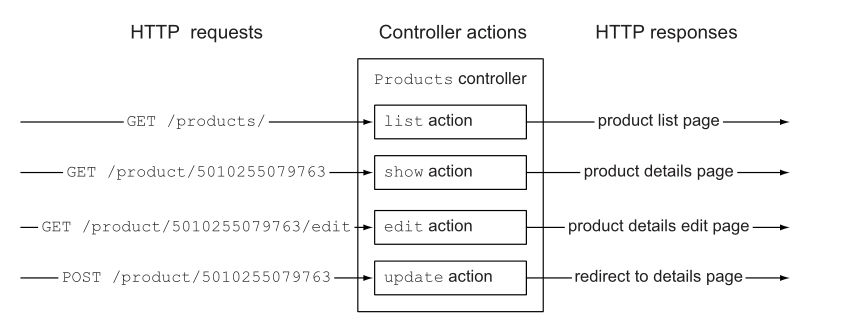
\includegraphics[scale=0.7]{Gambar/2_controllers1.PNG}
	\caption{Hubungan \textit{routes} dan \textit{controllers} dalam memproses HTTP \textit{requests}\cite{playforjava}}
	\label{fig:2_controllers1}
\end{figure}

Berikut adalah contoh penulisan program suatu kelas \textit{controllers}:

\begin{lstlisting}
package controllers;

import play.mvc.Controller;

public class Application extends Controller {

	public Result index() {
		return ok(index.render("Your new application is ready."));
	}

}
\end{lstlisting}

Penulisan kode pada suatu kelas \textit{controllers} menggunakan bahasa Java dan memiliki aturan khusus (contoh kode di atas). Aturan khusus dijelaskan ke dalam poin-poin sebagai berikut:
\begin{enumerate}
	\item \textit{Visibility} kelas dan \textit{method} pada kelas tersebut harus \textit{public} (baris 5),
	\item Kelas yang dibuat harus merupakan turunan dari ``\texttt{play.mvc.Controller}'' (baris 5),
	\item Nilai kembalian \textit{method} yang dibuat dalam suatu kelas \textit{controllers} harus berupa objek dari kelas Result (baris 7 dan 8).
\end{enumerate}
	
\subsection{\textit{Database}}
\label{sec:database}
Play Framework menyediakan sebuah \textit{plugin} yang dapat digunakan untuk mengatur koneksi JDBC ke berbagai jenis aplikasi \textit{database} yang tersedia\cite{playframeworkweb}. Salah satu koneksi \textit{database} yang disediakan oleh Play adalah koneksi ke MySQL. Secara \textit{default} \textit{plugin} yang disediakan oleh Play masih belum aktif. Perlu dilakukan beberapa langkah agar \textit{plugin} tersebut dapat aktif. Berikut adalah langkah-langkah yang dilakukan agar Play Framework dapat terhubung dengan \textit{database} MySQL:
\begin{enumerate}
	\item Menambahkan kode program ke dalam ``build.sbt'' (gambar \ref{fig:2_strukturplay}), yaitu:
	
	\begin{lstlisting}
	libraryDependencies += javaJdbc
	libraryDependencies += "mysql" % "mysql-connector-java" % "5.1.18"
	\end{lstlisting}
	
	Baris 1 kode program di atas adalah untuk mengaktifkan plugin JDBC pada Play Framework. Play tidak menyediakan \textit{database driver} apapun, untuk itu perlu menambahkan \textit{database driver} (baris 2) sebagai \textit{dependency} untuk aplikasi Play Framework.
	
	\item Menambahkan kode program ke dalam ``conf/application.conf'' (gambar \ref{fig:2_strukturplay}), yaitu:
	
	\begin{lstlisting}
	db.default.driver=com.mysql.jdbc.Driver
	db.default.url="jdbc:mysql://localhost/playdb"
	db.default.username=playdbuser
	db.default.password="a strong password"
	\end{lstlisting}
	
	Baris 1 kode program di atas menyatakan jenis \textit{driver} yang digunakan, yaitu MySQL. Baris 2 kode program menyatakan nama database yang digunakan, yaitu ``playdb''. Baris 3 dan 4 menyatakan \textit{username} dan \textit{password} yang dibutuhkan dalam otentikasi terhadap \textit{server database} untuk mendapatkan hak akses tertentu terhadap \textit{database}.
\end{enumerate}

	Salah satu aktivitas programming yang dibantu JDBC adalah menghubungkan aplikasi Java ke suatu sumber data seperti \textit{database} (subbab \ref{sec:jdbc}). Play Framework telah menyediakan kelas ``DB'' yang dapat memudahkan aplikasi Java membuat suatu koneksi dengan \textit{database}. Berikut adalah contoh kode yang diperlukan untuk menggunakan kelas ``DB'' dari Play Framework:
	\begin{lstlisting}
	import play.db.*;

	Connection connection = DB.getConnection();
	\end{lstlisting}
	Contoh kode di atas menyederhanakan penulisan kode milik JDBC (contoh kode pada subbab \ref{sec:jdbc} baris 3-6). 
	
\section{JSON}
\label{sec:json}
JSON (\textit{JavaScript Object Notation}) adalah sebuah format pertukaran data ringan\cite{json}. JSON dapat dibangun dalam 2 buah struktur:
\begin{enumerate}
	\item Sekumpulan pasangan antara nama dengan nilai. Umumnya dikenal dengan sebutan objek. Sebuah objek dalam JSON dimulai dengan karakter ``\texttt{\{}'' dan diakhiri dengan karakter ``\texttt{\}}''. Diantara karkater ``\texttt{\{}'' dan ``\texttt{\}}'' dapat disisipkan sekumpulan pasangan ``\texttt{nama:nilai}'' yang dipisahkan dengan karakter ``\texttt{,}''.
	\item Sekumpulan data terstruktur. Umumnya dikenal dengan sebutan \textit{array}. Sebuah \textit{array} dalam JSON dimulai dengan karakter ``\texttt{[}'' dan diakhiri dengan karakter ``\texttt{]}''. Diantara karkater ``\texttt{[}'' dan ``\texttt{]}'' dapat disisipkan sekumpulan data (dapat berupa nilai, objek atau \textit{array}) yang dipisahkan dengan karakter ``\texttt{,}''. Dalam \textit{array}. Setiap data dalam \textit{array} tidak harus sama jenisnya.
\end{enumerate}

Nilai dalam JSON dapat berupa \textit{string} (sekumpulan karakter yang diapit dengan 2 tanda kutip ganda, contoh: ``\texttt{karakter}''), angka, \texttt{true}, \texttt{false}, atau \texttt{null}.

Berikut adalah contoh sebuah data JSON:
\begin{lstlisting}
	{
		"status":"error",
		"message":"Value of userid is expected but not found"
	}
\end{lstlisting}

Contoh kode di atas adalah sebuah objek (baris 1-4) yang memiliki 2 buah pasangan ``\texttt{nama:nilai}'' yang dipisahkan oleh karakter ``\texttt{,}'' (baris 2-3). Contoh di atas juga menggunakan \textit{string} sebagai nilainya (baris 2 dan 3).

\section{\textit{Regular Expression}}
\label{sec:regex}
Sebuah \textit{regular expression} (\textit{regex}) adalah karakter atau kata istimewa yang dapat digunakan untuk melakukan pola pencarian tertentu.